\chapter{NodeHandler}
The \textit{NodeHandler} is the main entry point when you require RootJS by using
\begin{verbatim}
// JavaScript: Load ROOT bindings in JavaScript
var root = require(rootJS.node);

// C++: Expose the initialize method as the main entry point
NODE_MODULE(rootJS, initialize)
\end{verbatim}
\begin{figure}[H]
	\centering
	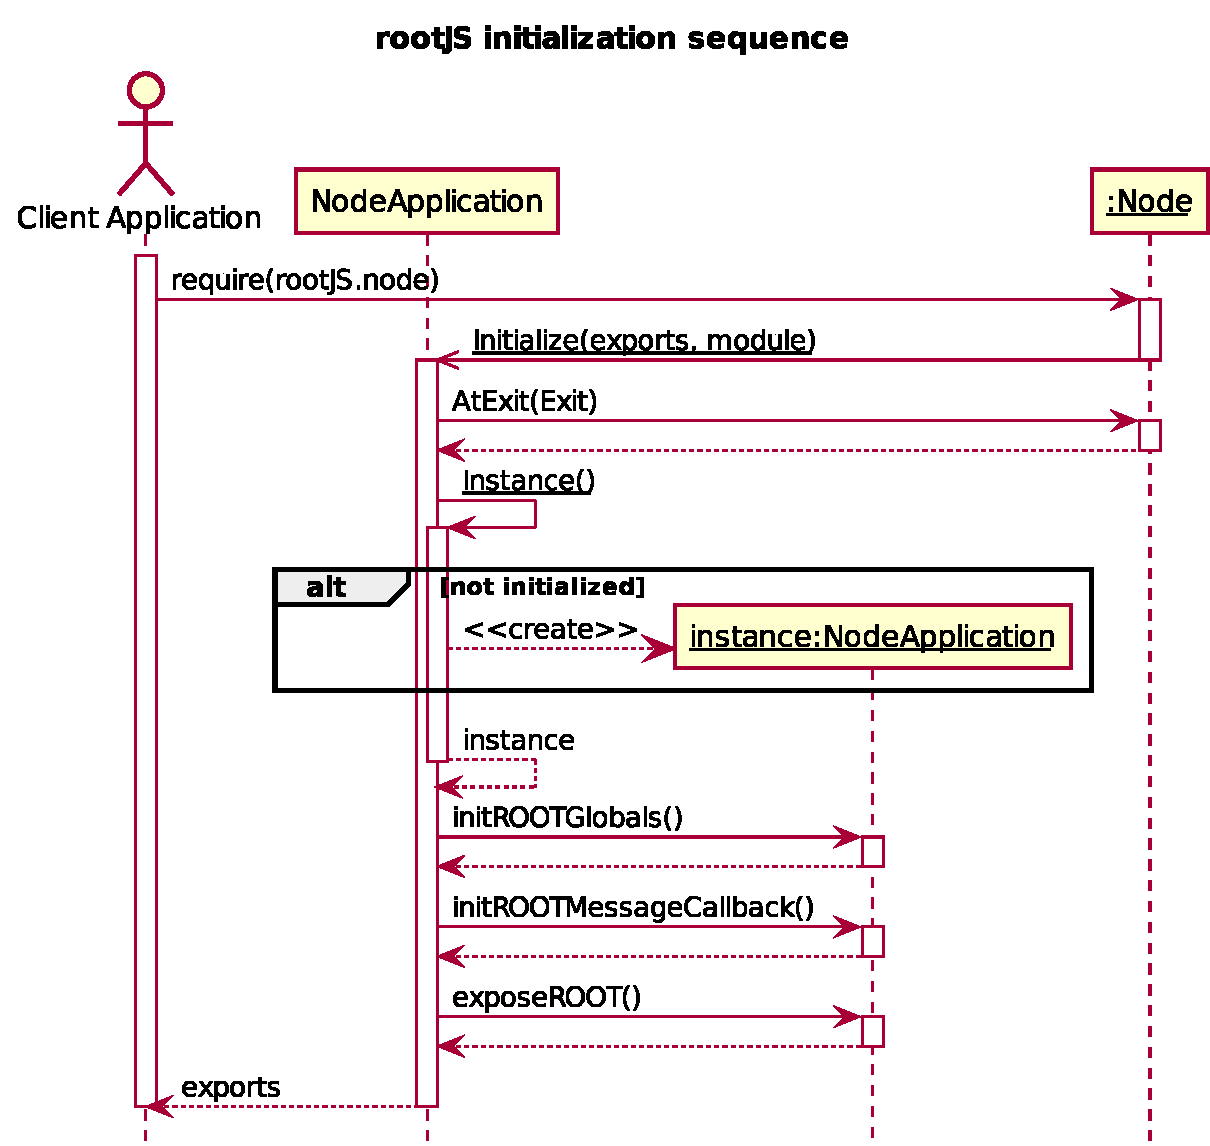
\includegraphics[width=18cm]{./latex/resources/initSequence.pdf}
	\caption{initialization sequence}
\end{figure}
After running the \textit{initialize} method ROOT is fully initialized and all features are exposed to JavaScript.
\begin{figure}[H]
	\centering
	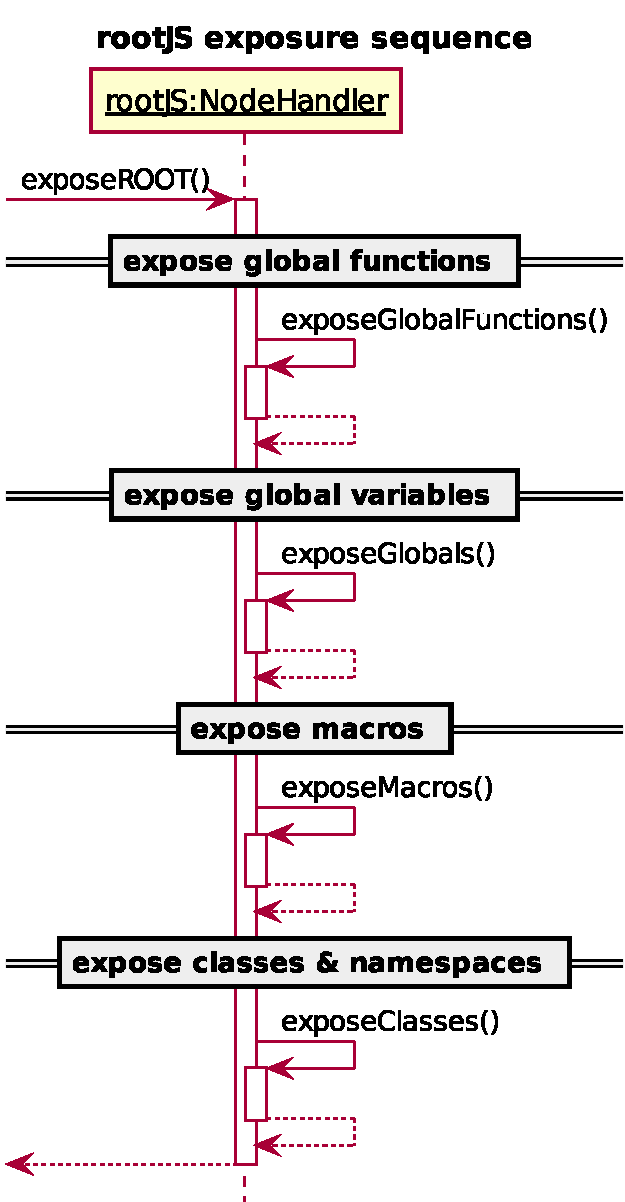
\includegraphics[width=10cm]{./latex/resources/exposureSequence.pdf}
	\caption{class exposure sequence}
\end{figure} \pagebreak
\section{initialize}
\begin{longtable}{p{3cm} @{\hskip 1cm} p{12cm}}
 \hline
\textit{Name} & \texttt{NodeHandler::initialize(exports: Local<Object>, module: Local<Object>)}\\
\hline
 \textit{Visibility} & public static\\
\hline
\textit{Parameters} & \textit{exports: Local<Object>, module: Local<Object>} parameters passed by Node.JS\\
\hline
\textit{Return value} & \textit{none} The features will be exported by passing them to the exports parameter \\
  \hline
 \textit{Behavior} & This will create an instance of \textit{NodeApplication} and store it in gApplication, to ensure that all ROOT functionality that relies on gApplication will function properly.
 Furthermore this will run \textit{getExports} to retrieve the features to be exported to JavaScript. This will then be put into the exports object which has been passed to this method \\
\hline
\end{longtable}
\section{getExports}
\begin{longtable}{p{3cm} @{\hskip 1cm} p{12cm}}
 \hline
\textit{Name} & \texttt{NodeHandler::getExports()}\\
\hline
 \textit{Visibility} & public\\
\hline
\textit{Parameters} & \textit{none}\\
\hline
\textit{Return value} & \textbf{Local<Object>} features to be exported \\
  \hline
 \textit{Behavior} & This method will run multiple private methods to collect global functions, global variables, macros and classes.
 All these items will be stored in a v8 object which will be passed to RootJS via the initialize method. \\
\hline
\end{longtable} \pagebreak
